% (c) 2012 Silvia Cibola - silvia.cibola@gmail.com
% (c) 2012-2014 Dimitrios Vrettos - d.vrettos@gmail.com
% (c) 2015 Daniele Zambelli daniele.zambelli@gmail.com

\chapter{Vettori}

\section{Prime definizioni}
\label{sec:vett_primedefinizioni}

% \begin{wrapfloat}{figure}{r}{0pt}
% \includegraphics[scale=0.35]{img/fig000_.png}
% \caption{...}
% \label{fig:...}
% \end{wrapfloat}
% 
% \begin{center} \input{\folder lbr/fig000_.pgf} \end{center}

Sappiamo che due punti~$A$ e~$B$ presi su una retta~$a$ determinano il 
segmento~$b$ di estremi~$A$ e~$B$ fissiamo su di esso un verso di percorrenza, 
per esempio da~$A$ verso~$B$.
\begin{definizione}
Il \emph{segmento orientato} di estremi~$A$ e~$B$ si chiama \emph{vettore}; 
esso viene indicato con~$\overrightarrow{AB}$ oppure con~$\vec{u}$
il punto~$A$ è il primo estremo e~$B$ il secondo estremo.
\end{definizione}
Un \emph{vettore libero} è caratterizzato da tre elementi:
\begin{itemize*}
\item la \emph{direzione} indicata dalla retta su cui giace;
\item il \emph{verso} indicato dalla punta della freccia che dal primo estremo 
va al secondo estremo;
\item il \emph{modulo o intensità}, uguale alla misura del segmento~$AB$: 
scriveremo~$|\vec{u}|=\overline{AB}$ e leggeremo "il modulo del 
vettore~$\vec{u}$ è
uguale alla misura del segmento~$AB$".
\end{itemize*}
Un \emph{vettore applicato} è caratterizzato oltre che dai tre elementi 
suddetti anche dal punto di applicazione,
ovvero il punto da cui parte la freccia, chiamato anche primo estremo del 
vettore.

\begin{exrig}
\begin{esempio}
I due vettori~$\overrightarrow{AB}$ e~$\overrightarrow{DC}$ in figura 
\ref{fig:F.1} appartengono alla stessa retta, quindi hanno stessa direzione, 
verso opposto e modulo diverso.
\end{esempio}

\begin{esempio}
I due vettori~$\overrightarrow{AB}$ e~$\overrightarrow{DC}$ in figura 
\ref{fig:F.2} appartengono a rette parallele, quindi hanno stessa direzione. I 
loro versi sono opposti e hanno
uguale intensità: essi si chiamano \emph{vettori opposti} e 
scriveremo~$\overrightarrow{AB}=-\overrightarrow{DC}$.
\end{esempio}

\begin{esempio}
I due vettori~$\overrightarrow{AB}$ e~$\overrightarrow{CD}$ in figura 
\ref{fig:F.3} appartengono a rette parallele, quindi hanno stessa direzione. 
Hanno lo stesso verso e uguale intensità:
essi si chiamano \emph{equipollenti} e 
scriveremo~$\overrightarrow{AB}=\overrightarrow{CD}$.
\end{esempio}
\end{exrig}

\begin{inaccessibleblock}[Figura: TODO]
 \begin{figure}[b]
\centering
% (c) 2012 Dimitrios Vrettos - d.vrettos@gmail.com


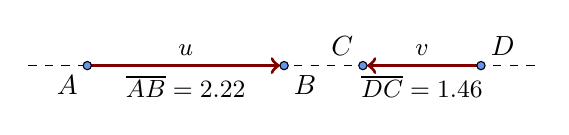
\begin{tikzpicture}[x=5mm,y=5mm]
\begin{scope}[dashed]

\draw (-1,0) -- (12,0);
\end{scope}
\begin{scope}[Maroon, very thick,->, shorten >=1.5pt]
\draw (.5,0) -- (5.5,0);
\draw  (10.5,0)--(7.5,0);
\end{scope}

\node [below left] at (.5,0) {$A$};
\node [below right] at (5.5,0) {$B$};
\node [above left] at (7.5,0) {$C$};
\node [above right] at (10.5,0) {$D$};

\begin{scope}[font=\small]
\node[below] at (9,0) {$\overline{DC}=1.46$};
\node[above] at (9,0) {$v$};
\node[below] at (3,0) {$\overline{AB}=2.22$};
\node[above] at (3,0) {$u$};
\end{scope}

\foreach \x in {.5,5.5,7.5,10.5}
\filldraw[fill=CornflowerBlue, draw=black] (\x,0) circle (1.5pt);
\end{tikzpicture}
\caption{I vettori hanno stessa direzione, verso opposto e modulo 
diverso.}\label{fig:F.1}
\end{figure}
\end{inaccessibleblock}


 \begin{inaccessibleblock}[Figura: TODO]
 \begin{figure}[t]
\begin{minipage}{0.45\textwidth}
\centering
% (c) 2012 Dimitrios Vrettos - d.vrettos@gmail.com

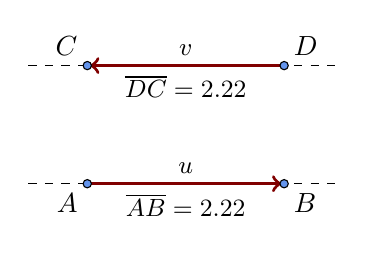
\begin{tikzpicture}[x=5mm,y=5mm]
  \begin{scope}[dashed]
    \foreach \y in {0,3}
      \draw (-1,\y) -- (7,\y);
  \end{scope}
  
  \begin{scope}[Maroon, very thick,->, shorten >=1pt]
    \draw (.5,0) -- (5.5,0);
    \draw (5.5,3) -- (.5,3) ;
  \end{scope}

  \node [below left] at (.5,0) {$A$};
  \node [below right] at (5.5,0) {$B$};
  \node [above left] at (.5,3) {$C$};
  \node [above right] at (5.5,3) {$D$};

  \begin{scope}[font=\small]
    \node[below] at (3,3) {$\overline{DC}=2.22$};
    \node[above] at (3,3) {$v$};
    \node[below] at (3,0) {$\overline{AB}=2.22$};
    \node[above] at (3,0) {$u$};
  \end{scope}

  \foreach \x in {.5,5.5}{
    \foreach \yi in {0,3}
      \filldraw[fill=CornflowerBlue, draw=black] (\x,\yi) circle (1.5pt);}
\end{tikzpicture}
\caption{Vettori opposti.}\label{fig:F.2}
\end{minipage}\hfil
\begin{minipage}{0.45\textwidth}
\centering
% (c) 2012 Dimitrios Vrettos - d.vrettos@gmail.com

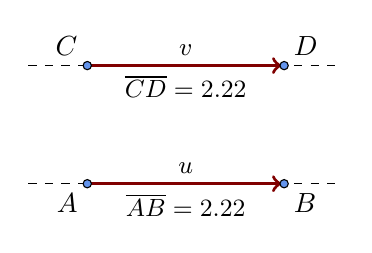
\begin{tikzpicture}[x=5mm,y=5mm]
  \begin{scope}[dashed]
    \foreach \y in {0,3}
      \draw (-1,\y) -- (7,\y);
  \end{scope}
  
  \begin{scope}[Maroon, very thick,->, shorten >=1pt]
    \draw (.5,0) -- (5.5,0);
    \draw (.5,3) -- (5.5,3);
  \end{scope}

  \node [below left] at (.5,0) {$A$};
  \node [below right] at (5.5,0) {$B$};
  \node [above left] at (.5,3) {$C$};
  \node [above right] at (5.5,3) {$D$};

  \begin{scope}[font=\small]
    \node[below] at (3,3) {$\overline{CD}=2.22$};
    \node[above] at (3,3) {$v$};
    \node[below] at (3,0) {$\overline{AB}=2.22$};
    \node[above] at (3,0) {$u$};
  \end{scope}

  \foreach \x in {.5,5.5}{
    \foreach \yi in {0,3}
      \filldraw[fill=CornflowerBlue, draw=black] (\x,\yi) circle (1.5pt);}
\end{tikzpicture}
\caption{Vettori equipollenti.}\label{fig:F.3}
\end{minipage}
\end{figure}
\end{inaccessibleblock}

Osserviamo che un vettore può essere interpretato come uno spostamento dal 
primo estremo al secondo estremo, avente la direzione della retta cui appartiene 
il vettore stesso nel
verso indicato dalla freccia.
Nel piano dotato di riferimento cartesiano ortogonale (figura~\ref{fig:F.4}a) è 
rappresentato il vettore~$\overrightarrow{AB}$ avente il primo estremo nel 
punto~$A(-2;1)$ e
il secondo estremo
in~$B(1;2)$. Per andare da~$A$ a~$B$ si possono compiere diversi percorsi: 
possiamo procedere sul vettore~$\vec{u}$ oppure possiamo scegliere di compiere 
due spostamenti particolari,
uno parallelo all'asse~$x$ e l'altro parallelo all'asse~$y$. In tal modo si 
determina il punto~$C(1;1)$ come "tappa intermedia" per raggiungere~$B$:
ci spostiamo sul vettore~$\overrightarrow{AC}$ e poi da~$C$ sul 
vettore~$\overrightarrow{CB}$.

\begin{inaccessibleblock}[Figura: TODO]
 \begin{figure}[b]
\centering
% (c) 2012 Dimitrios Vrettos - d.vrettos@gmail.com

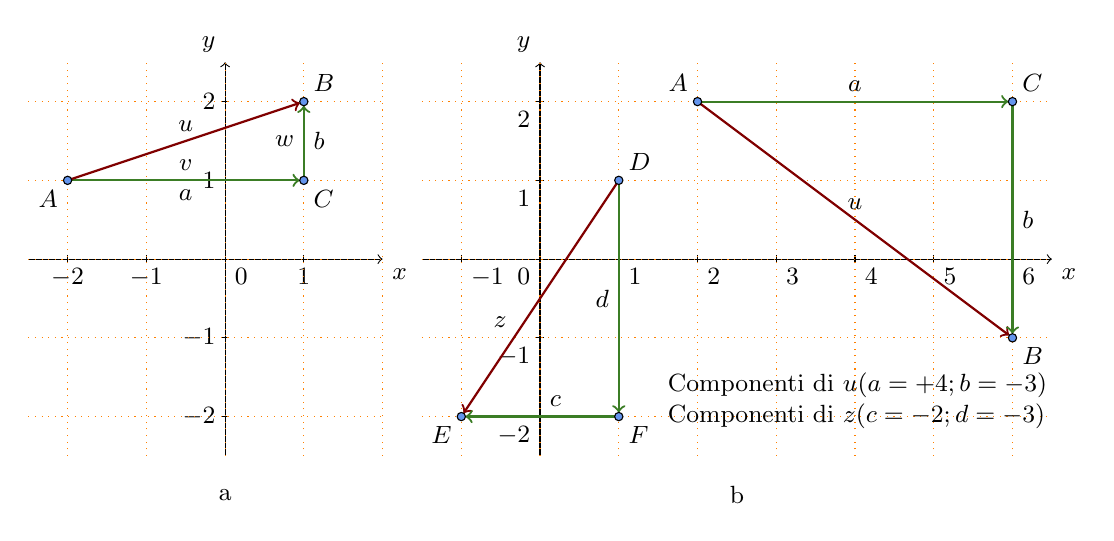
\begin{tikzpicture}[x=10mm,y=10mm, font=\small]

  \begin{scope}[->]
    \draw (-2.5,0) -- (2,0) node [below right] () {$x$};
    \draw (0,-2.5) -- (0,2.5) node[above left] {$y$};
  \end{scope}

  \foreach \x/\xtext in {-2/-2,-1/-1, 1/1}{
    \node[below] at (\x,0) {$\xtext$};
    \draw (\x,1.5pt) -- (\x,-1.5pt);}
  \foreach \y/\ytext in {-2/-2,-1/-1, 1/1, 2/2}{
    \node[left] at (0,\y) {$\ytext$};
    \draw (1.5pt,\y) -- (-1.5pt,\y);}
  \node[below right] at (0,0) {$0$};

  \node[below left] at (-2,1) {$A$};
  \node[above right] at (1,2) {$B$};
  \node[below right] at (1,1) {$C$};

  \node[above] at (-.5,1.5) {$u$};
  
  \node[above] at (-.5,1) {$v$};
  \node[below] at (-.5,1) {$a$};
  \node[left] at (1,1.5) {$w$};
  \node[right] at (1,1.5) {$b$};

\node at (0,-3) {a};
  \begin{scope}[dotted, orange]
    \draw (-2.5,-2.5) grid (2,2.5);
  \end{scope}

  \begin{scope}[thick, OliveGreen, shorten >=1.5pt, ->]
    \draw (-2,1) -- (1,1);
    \draw[Maroon] (-2,1) -- (1,2);
    \draw (1,1) -- (1,2);
  \end{scope}
  
  \begin{scope}[fill=CornflowerBlue, draw=black]
    \filldraw (-2,1) circle (1.5pt);
    \filldraw (1,2) circle (1.5pt);
    \filldraw (1,1) circle (1.5pt);
  \end{scope}

  \begin{scope}[xshift=40mm]
    \begin{scope}[->]
    \draw (-1.5,0) -- (6.5,0) node [below right] () {$x$};
    \draw (0,-2.5) -- (0,2.5) node[above left] {$y$};
    \end{scope}

    \foreach \x/\xtext in {-1/-1, 1/1,2/2,3/3,4/4,5/5,6/6}{
      \node[below right] at (\x,0) {$\xtext$};
      \draw (\x,1.5pt) -- (\x,-1.5pt);}
    \foreach \y/\ytext in {-2/-2,-1/-1, 1/1, 2/2}{
      \node[below left] at (0,\y) {$\ytext$};
      \draw (1.5pt,\y) -- (-1.5pt,\y);}
    \node[below left] at (0,0) {$0$};

    \node[above left] at (2,2) {$A$};
    \node[below right] at (6,-1) {$B$};
    \node[above right] at (6,2) {$C$};

    \node[above] at (4,2) {$a$};
    \node[right] at (6,.5) {$b$};
    \node[above] at (4,.5) {$u$};

    \node[above right] at (0,-2) {$c$};
    \node[left] at (1,-.5) {$d$};
    \node[left] at (-.3,-.8) {$z$};

    \node[above right] at (1,1) {$D$};
    \node[below right] at (1,-2) {$F$};
    \node[below left] at (-1,-2) {$E$};

    \node at (2.5,-3) {b};
    \begin{scope}[dotted, orange]
      \draw (-1.5,-2.5) grid (6.5,2.5);
    \end{scope}

    \begin{scope}[thick, shorten >=1.5pt, ->]
      \begin{scope}[Maroon]
	\draw(2,2) -- (6,-1);
	\draw (1,1) -- (-1,-2);
      \end{scope}
      
      \begin{scope}[OliveGreen]
	\draw(2,2) -- (6,2);
	\draw (6,2) -- (6,-1);

	\draw (1,1) -- (1,-2);
	\draw (1,-2) -- (-1,-2);
	\end{scope}
    \end{scope}

    \begin{scope}[fill=CornflowerBlue, draw=black]
      \filldraw (6,2) circle (1.5pt);
      \filldraw (2,2) circle (1.5pt);
      \filldraw (6,-1) circle (1.5pt);

      \filldraw (1,1) circle (1.5pt);
      \filldraw (1,-2) circle (1.5pt);
      \filldraw (-1,-2) circle (1.5pt);
    \end{scope}

    \node[right] () at (1.5,-1.6) {Componenti di $u(a=+4;b=-3)$};
    \node[right] () at (1.5,-2) {Componenti di $z(c=-2;d=-3)$};
  \end{scope}
\end{tikzpicture}
\caption{Spostamenti di vettori.}\label{fig:F.4}
\end{figure}
\end{inaccessibleblock}


\begin{definizione}
Chiamiamo \emph{componenti} del vettore~$\overrightarrow{AB}$ le \emph{misure 
con segno} dei segmenti~$AC$ e~$CB$ con la precisazione di assegnare il 
segno~$+$ alle misure
dello spostamento avente lo stesso verso degli assi coordinati e segno~$-$ se 
il verso è opposto a quello degli assi coordinati.
\end{definizione}

In figura \ref{fig:F.4} a le componenti del vettore assegnato sono positive in 
quanto sia lo spostamento orizzontale che quello verticale avvengono nello 
stesso
verso degli assi coordinati. Scriveremo~$\overrightarrow{AB}(+3;+1)$. Tutti i 
vettori del piano cartesiano di componenti~$(+3,+1)$ sono equipollenti 
a~$\overrightarrow{AB}$.
Ciò che li distingue in modo univoco è il loro punto di applicazione.

% \begin{exrig}
\begin{esempio}
Il vettore~$\vec{z}$ della figura \ref{fig:F.4} b ha componenti entrambe 
negative poiché lo spostamento orizzontale e quello verticale avvengono in verso
contrario rispetto al verso degli assi coordinati: scriveremo~$\vec{z}(-2;-3)$. 
Il vettore~$\vec{u}$ della figura \ref{fig:F.4} b ha la componente
lungo l'asse~$x$ positiva e negativa la componente verticale: 
scriveremo~$\vec{u}(+4;-3)$.
\end{esempio}
% \end{exrig}

\begin{procedura}
Determinare le componenti cartesiane di un vettore~$\vec{v}$, note le 
coordinate cartesiane degli estremi~$A(x_A;y_A)$ e~$B(x_B;y_B)$:
\begin{enumeratea}
\item dal primo estremo tracciamo la parallela all'asse~$x$ e dal secondo 
estremo la parallela all'asse~$y$ determinando il punto~$C(x_B;y_A)$
\item calcoliamo le misure con segno~$a=x_B-x_A$ $b=y_B-y_A$
\item scriviamo~$\vec{v}(a;b)$.
\end{enumeratea}
\end{procedura}
Ottenute le componenti si determina il \emph{modulo del vettore} utilizzando il 
teorema di Pitagora; si ha infatti~$|\vec{u}|=\overline{AB}=\sqrt{a^2+b^2}$.
Il rapporto~$m_{\vec{u}}=\frac{b}{a}$ indica la \emph{direzione del vettore}.

% \begin{exrig}
\begin{esempio}
Assegnato il vettore della figura, determinate le sue componenti, il modulo e 
la direzione. Completate i passi indicati nella strategia risolutiva:
\begin{multicols}{2}
 \begin{itemize*}
\item scrivete le coordinate degli estremi del vettore 
assegnato~$A(\ldots;\ldots)$ e~$B(\ldots;\ldots)$
\item individuate le componenti del vettore~$\vec{w}$:
\begin{itemize*}
\item segnate il punto~$C$ calcolate $a=x_B-x_A$ e~$b=y_B-y_A$
\item le componenti del vettore sono $\vec{w}(\ldots;\ldots)$
\end{itemize*}
\item determinate il modulo del vettore~$|\vec{w}|=\sqrt{\ldots}$
\item determinate la direzione del vettore~$m_{\vec{w}}=\ldots$.
\end{itemize*}
\begin{center}
 % (c) 2012 Dimitrios Vrettos - d.vrettos@gmail.com

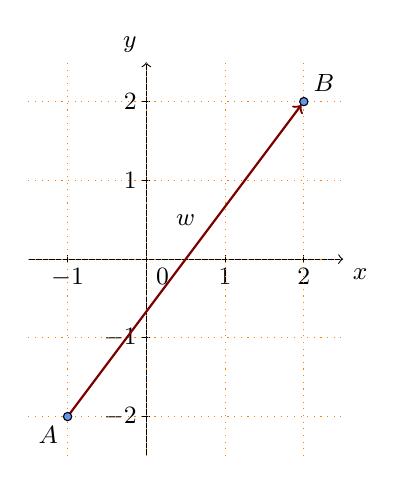
\begin{tikzpicture}[x=10mm,y=10mm, font=\small]

  \begin{scope}[->]
   \draw (-1.5,0) -- (2.5,0) node[below right] {$x$};
    \draw (0,-2.5) -- (0,2.5) node[above left] {$y$};
  \end{scope}

  \foreach \x/\xtext in {-1/-1, 1/1,2/2}{
    \node[below] at (\x,0) {$\xtext$};
    \draw (\x,1.5pt) -- (\x,-1.5pt);}
  \foreach \y/\ytext in {-2/-2,-1/-1, 1/1, 2/2}{
    \node[left] at (0,\y) {$\ytext$};
    \draw (1.5pt,\y) -- (-1.5pt,\y);}
  \node[below right] at (0,0) {$0$};

  \begin{scope}[dotted, orange]
    \draw (-1.5,-2.5) grid (2.5,2.5);
  \end{scope}

  \begin{scope}[thick, Maroon, shorten >=1.5pt, ->]
    \draw (-1,-2) -- (2,2);
      \end{scope}
  
\begin{scope}[fill=CornflowerBlue, draw=black]
\filldraw (2,2) circle (1.5pt) node[above right] {$B$};
\filldraw (-1,-2) circle (1.5pt) node[below left] {$A$};
\end{scope}

\node at (.5,.5) {$w$};

\end{tikzpicture}

\end{center}
\end{multicols}
\end{esempio}

\begin{esempio}
\begin{multicols}{2}
 Tracciate nel riferimento cartesiano ortogonale il vettore~$\vec{v}(1;-3)$. 
Nella richiesta di questo quesito sembra manchi qualcosa: conosciamo
le componenti del vettore, ma dove mettiamo il primo estremo? Provate a mettere 
il primo estremo in ciascuno dei seguenti punti:~$A_1(-1;2)$ $A_2(1;0)$ 
$A_3(3;-2)$
e determinate il secondo estremo di ciascun vettore; completate indicando per 
ciascuno il modulo e la direzione. È vero che tutti i vettori tracciati sono 
equipollenti?
In figura è rappresentato il vettore equipollente a quelli costruiti avente il 
primo estremo nell'origine del riferimento.
\begin{center}
 % (c) 2012 Dimitrios Vrettos - d.vrettos@gmail.com

\begin{tikzpicture}[x=10mm,y=10mm, font=\small]

  \begin{scope}[->]
    \draw (-1.5,0) -- (2.5,0) node [below right] () {$x$};
    \draw (0,-3.5) -- (0,1.5) node[above left] {$y$};
  \end{scope}

  \foreach \x/\xtext in {-1/-1, 1/1,2/2}{
    \node[below] at (\x,0) {$\xtext$};
    \draw (\x,1.5pt) -- (\x,-1.5pt);}
  \foreach \y/\ytext in {-3/-3,-2/-2,-1/-1, 1/1}{
    \node[left] at (0,\y) {$\ytext$};
    \draw (1.5pt,\y) -- (-1.5pt,\y);}
  \node[below left] at (0,0) {$0$};

  \begin{scope}[dotted, orange]
    \draw (-1.5,-3.5) grid (2.5,1.5);
  \end{scope}

  \begin{scope}[thick, Maroon, shorten >=1.5pt, ->]
    \draw (-0,0) -- (1,-2);
      \end{scope}
  
\begin{scope}[fill=CornflowerBlue, draw=black]
\filldraw (1,-2) circle (1.5pt) node[below right] {$B$};
\filldraw (0,0) circle (1.5pt) node[above left] {$A$};
\end{scope}

\node at (.8,-1) {$u$};

\end{tikzpicture}
\end{center}

\end{multicols}

\osservazione
Quando si assegna un vettore mediante le sue componenti, collocheremo il primo 
estremo
nell'origine del riferimento cartesiano ortogonale e il secondo estremo (punta 
della freccia) avrà come
coordinate le componenti del vettore in questione.
\end{esempio}
% \end{exrig}

% \ovalbox{\risolvi \ref{ese:F.1}}

\section{Operazioni con i vettori}
\label{sec:vett_operazioni}

\subsection{Somma di vettori}
\begin{definizione}
Nel punto~$A$ del piano sono applicati due vettori~$\vec{u}$ e~$\vec{v}$: 
dall'estremo~$B$ si
traccia la retta parallela ad~$AC$ e da~$C$ la parallela ad~$AB$ e si indica 
con~$D$ il loro punto di intersezione.
Il vettore~$AD$ individuato dalla diagonale~$AD$ del parallelogrammo è la 
\emph{somma dei vettori}~$u$ e~$v$, e si scrive~$w=u+v$.
\end{definizione}


\begin{inaccessibleblock}[Somma di due vettori con la regola del 
  parallelogramma.]
 \begin{figure}[h]
\centering
% (c) 2012 Dimitrios Vrettos - d.vrettos@gmail.com

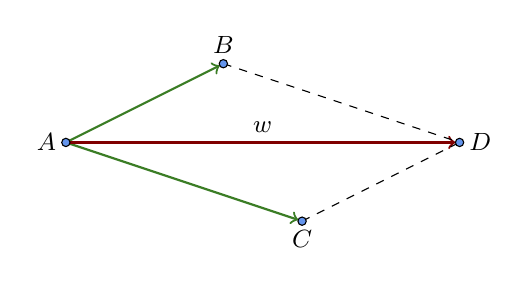
\begin{tikzpicture}[x=10mm,y=10mm, font=\small]

  \begin{scope}[thick,shorten >=1.5pt, ->]
    \begin{scope}[OliveGreen]
      \draw (0,0) -- (2,1);
      \draw (0,0) -- (3,-1);
    \end{scope}  
    
    \begin{scope}[Maroon]
      \draw (0,0) -- (5,0);
    \end{scope}
  \end{scope}

  \begin{scope}[dashed]
    \draw[xshift=30mm,yshift=-10mm] (0,0) -- (2,1);
    \draw[xshift=20mm,yshift=10mm] (0,0) -- (3,-1);
  \end{scope}

  \begin{scope}[fill=CornflowerBlue, draw=black]
    \filldraw (5,0) circle (1.5pt) node[right] {$D$};
    \filldraw (0,0) circle (1.5pt) node[left] {$A$};
    \filldraw (2,1) circle (1.5pt) node[above] {$B$};
    \filldraw (3,-1) circle (1.5pt) node[below] {$C$};
  \end{scope}

  \node[above] at (2.5,0) {$w$};

\end{tikzpicture}
 \caption{Somma di due vettori.}
 \label{fig:vett_somma_parallelogramma}
\end{figure}
\end{inaccessibleblock}

Nella sua opera \emph{Philosophiae naturalis principia mathematica} del~1682, 
Isaac Newton (1642-1727) nel primo corollario alle leggi del moto,
scrive: <<un corpo spinto da due forze congiunte descriverà la diagonale di un 
parallelogrammo nello stesso tempo nel quale descriverebbe separatamente i 
lati>>.

% \vspazio\ovalbox{\risolvi \ref{ese:F.2}}

Illustriamo con un esempio che vale anche la \emph{proprietà associativa}.

% \begin{exrig}
\begin{esempio}
Dimostriamo che vale~$\vec{u}+(\vec{v}+\vec{w})=(\vec{u}+\vec{v})+\vec{w}$.
Nella figura \ref{fig:F.6} è realizzata la 
costruzione~$\vec{v}+\vec{w}=\vec{k}$ e~$\vec{u}+\vec{k}=\vec{j}$.
Nella figura \ref{fig:F.7} è realizzata la 
costruzione~$\vec{u}+\vec{v}=\vec{z}$ e~$\vec{z}+\vec{w}=\vec{j}$.
Sovrapponendo le due figure si può constatare che i vettori~$\vec{j}$ 
risultanti coincidono.
\end{esempio}
% \end{exrig}

\begin{inaccessibleblock}[Proprietà associativa della addizione tra vettori.]
 \begin{figure}[t]
\begin{minipage}{.45\textwidth}
 \centering
 % (c) 2012 Dimitrios Vrettos - d.vrettos@gmail.com

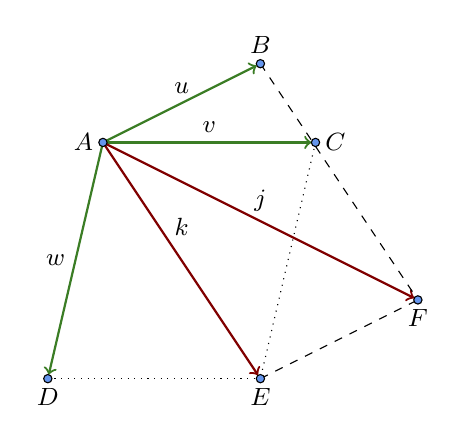
\begin{tikzpicture}[x=10mm,y=10mm, font=\small]

  \begin{scope}[thick,shorten >=1.5pt, ->]
    \begin{scope}[OliveGreen]
      \draw (0,0) -- (2,1); % vettore u
      \draw (0,0) -- (2.7,0); % vettore v
      \draw (0,0) -- (-.7,-3); % vettore w
    \end{scope}  
    
    \begin{scope}[Maroon]
      \draw (0,0) -- (4,-2); % vettore j
      \draw (0,0) -- (2,-3); % vettore k    
    \end{scope}
  \end{scope}

  \begin{scope}[dashed]
    \draw[xshift=20mm,yshift=-30mm] (0,0) -- (2,1);
    \draw[xshift=20mm,yshift=10mm] (0,0) -- (2,-3);
  \end{scope}

  \begin{scope}[dotted]
    \draw[xshift=-7mm,yshift=-30mm] (0,0) -- (2.7,0);
    \draw[xshift=27mm,yshift=0mm] (0,0) -- (-.7,-3);
  \end{scope}  

  \begin{scope}[fill=CornflowerBlue, draw=black]
    \filldraw (0,0) circle (1.5pt) node[left] {$A$};
    \filldraw (2,1) circle (1.5pt) node[above] {$B$};
    \filldraw (2,-3) circle (1.5pt) node[below] {$E$};
    \filldraw (4,-2) circle (1.5pt) node[below] {$F$};
    \filldraw (-.7,-3) circle (1.5pt) node[below] {$D$};
    \filldraw (2.7,0) circle (1.5pt) node[right] {$C$};
  \end{scope}

  \node[above] at (1,.5) {$u$};
  \node[above] at (1.35,0) {$v$};
  \node[above] at (2,-1) {$j$};
  \node[above] at (1,-1.3) {$k$};
  \node at (-.6,-1.5) {$w$};

\end{tikzpicture}
 \caption{$\vec{v}+\vec{w}=\vec{k}$ e~$\vec{u}+\vec{k}=\vec{j}$.}
 \label{fig:F.6}
\end{minipage}\hfil
\begin{minipage}{.45\textwidth}
 \centering
 % (c) 2012 Dimitrios Vrettos - d.vrettos@gmail.com

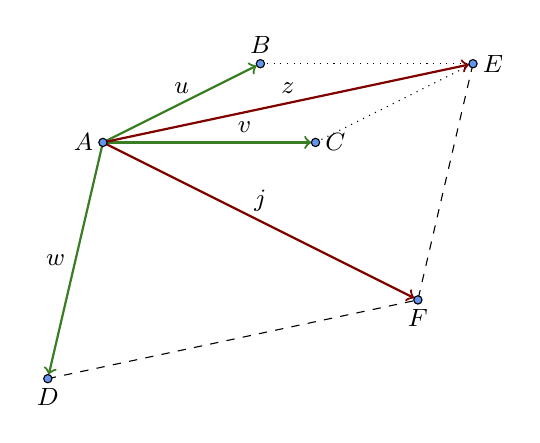
\begin{tikzpicture}[x=10mm,y=10mm, font=\small]

  \begin{scope}[thick,shorten >=1.5pt, ->]
    \begin{scope}[OliveGreen]
      \draw (0,0) -- (2,1); % vettore u
      \draw (0,0) -- (2.7,0); % vettore v
      \draw (0,0) -- (-.7,-3); % vettore w
    \end{scope}
    
    \begin{scope}[Maroon]
      \draw (0,0) -- (4,-2); % vettore j
      \draw (0,0) -- (4.7,1); % vettore z    
    \end{scope}
  \end{scope}

  \begin{scope}[dashed]
    \draw[xshift=47mm,yshift=10mm] (0,0) -- (-.7,-3);
    \draw[xshift=-7mm,yshift=-30mm] (0,0) -- (4.7,1);
  \end{scope}

  \begin{scope}[dotted]
    \draw[xshift=20mm,yshift=10mm] (0,0) -- (2.7,0);
    \draw[xshift=27mm,yshift=0mm] (0,0) -- (2,1);
  \end{scope}  

  \begin{scope}[fill=CornflowerBlue, draw=black]
    \filldraw (0,0) circle (1.5pt) node[left] {$A$};
    \filldraw (2,1) circle (1.5pt) node[above] {$B$};
    \filldraw (4.7,1) circle (1.5pt) node[right] {$E$};
    \filldraw (4,-2) circle (1.5pt) node[below] {$F$};
    \filldraw (-.7,-3) circle (1.5pt) node[below] {$D$};
    \filldraw (2.7,0) circle (1.5pt) node[right] {$C$};
  \end{scope}

  \node[above] at (1,.5) {$u$};
  \node[above] at (1.8,0) {$v$};
  \node[above] at (2,-1) {$j$};
  \node[above] at (2.35,.5) {$z$};
  \node at (-.6,-1.5) {$w$};

\end{tikzpicture}
 \caption{$\vec{u}+\vec{v}=\vec{z}$ e~$\vec{z}+\vec{w}=\vec{j}$.}
 \label{fig:F.7}
\end{minipage}
\end{figure}
\end{inaccessibleblock}

Osserviamo che la validità della proprietà associativa ci permette di costruire 
la somma di più vettori. Per come è definita l'operazione di somma, pensando al
vettore come rappresentante di uno spostamento dal primo estremo al secondo, 
possiamo interpretare la figura \ref{fig:vett_somma_parallelogramma} come 
lo spostamento di un punto prima da~$A$ fino a~$B$ e poi da questo fino a~$D$, 
essendo~$\vec{BD}$ un vettore equipollente ad~$\overrightarrow{AC}$. 
Quindi possiamo affermare che il vettore somma di due 
vettori~$\vec{u}$ e~$\vec{v}$ si può determinare prendendo due 
vettori~$\overrightarrow{AB}$ e~$\overrightarrow{BC}$ rispettivamente 
equipollenti
ai dati; se~$\overrightarrow{AB} \equiv \vec{u}$ e~$\overrightarrow{BC} \equiv 
\vec{v}$ (figura \ref{fig:F.8}), allora la somma è il 
vettore~$\overrightarrow{AC}$, avente~$A$
come primo estremo e~$C$,
ultimo estremo del secondo vettore, come secondo estremo.

Pertanto la somma di più vettori si può semplicemente determinare scegliendo 
per ogni addendo il vettore equipollente avente il primo estremo nell'estremo 
finale
dell'addendo precedente: la somma è il vettore avente il primo estremo nel 
punto iniziale del primo addendo e l'estremo finale nel secondo estremo 
dell'ultimo addendo.
% \begin{exrig}
\begin{esempio}
Somma di più vettori:~$\vec{z}+\vec{a}+\vec{b}+\vec{c}=\vec{s}$, (figura 
\ref{fig:F.9}).
\end{esempio}
% \end{exrig}

\begin{inaccessibleblock}[Figura: TODO]
 \begin{figure}[b]
\begin{minipage}[t]{.45\textwidth}
 \centering
 % (c) 2012 Dimitrios Vrettos - d.vrettos@gmail.com

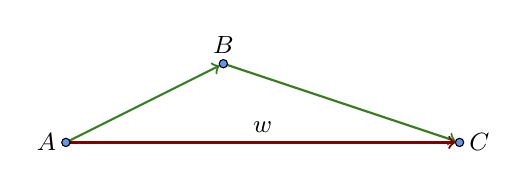
\begin{tikzpicture}[x=10mm,y=10mm, font=\small]

  \begin{scope}[thick,shorten >=1.5pt, ->]
    \begin{scope}[OliveGreen]
      \draw (0,0) -- (2,1);
      \draw (2,1) -- (5,0);
    \end{scope}  
    
    \begin{scope}[Maroon]
      \draw (0,0) -- (5,0);
    \end{scope}
  \end{scope}


  \begin{scope}[fill=CornflowerBlue, draw=black]
    \filldraw (5,0) circle (1.5pt) node[right] {$C$};
    \filldraw (0,0) circle (1.5pt) node[left] {$A$};
    \filldraw (2,1) circle (1.5pt) node[above] {$B$};
  \end{scope}

  \node[above] at (2.5,0) {$w$};

\end{tikzpicture}
 \caption{Somma di due vettori.}
 \label{fig:F.8}
\end{minipage}\hfil
\begin{minipage}[t]{.45\textwidth}
 \centering
 % (c) 2012 Dimitrios Vrettos - d.vrettos@gmail.com

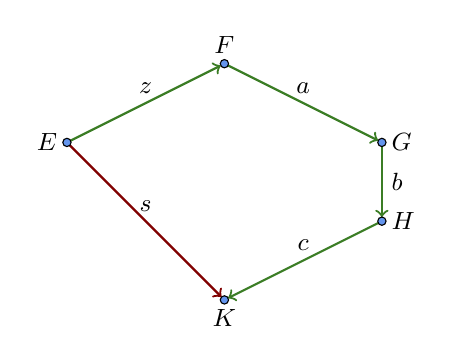
\begin{tikzpicture}[x=10mm,y=10mm, font=\small]

  \begin{scope}[thick,shorten >=1.5pt, ->]
    \begin{scope}[OliveGreen]
\draw (-2,2) -- (0,3);
\draw (0,3) -- (2,2);
\draw (2,2) -- (2,1);
\draw (2,1) -- (0,0);
    \end{scope}  
    
    \begin{scope}[Maroon]
      \draw (-2,2) -- (0,0);
    \end{scope}
  \end{scope}


  \begin{scope}[fill=CornflowerBlue, draw=black]
    \filldraw (-2,2) circle (1.5pt) node[left] {$E$};
    \filldraw (0,3) circle (1.5pt) node[above] {$F$};
    \filldraw (2,2) circle (1.5pt) node[right] {$G$};
    \filldraw (2,1) circle (1.5pt) node[right] {$H$};
    \filldraw (0,0) circle (1.5pt) node[below] {$K$};
  \end{scope}

  \node[above] at (-1,2.5) {$z$};
  \node[above] at (1,2.5) {$a$};
  \node[right] at (2,1.5) {$b$};
  \node[above] at (1,.5) {$c$};
  \node[above] at (-1,1) {$s$};

\end{tikzpicture}
 \caption{Somma di più vettori.}
 \label{fig:F.9}
\end{minipage}
\end{figure}
\end{inaccessibleblock}

Abbiamo visto come si costruisce geometricamente il vettore somma di vettori; 
vediamo come si determinano le componenti del vettore somma se la questione
è posta nel riferimento cartesiano ortogonale.

% \begin{exrig}
\begin{esempio}
Nel piano dotato di riferimento cartesiano ortogonale (figura~\ref{fig:F.10}) 
costruiamo il vettore somma dei vettori~$\vec{u}(1;2)$ e~$\vec{v}(3;-1)$ e 
determiniamone
le componenti.

Strategia risolutiva:
\begin{enumeratea}
\item costruiamo il vettore~$\vec{w}$ equipollente al vettore~$\vec{v}$ 
applicato al punto~$A$
\item determiniamo il punto$D(4;1)$
\item costruiamo il vettore~$\vec{z}=\vec{u}+\vec{v}$ di 
coordinate~$\vec{z}(4;1)$.
\end{enumeratea}
Osserviamo che il primo passo realizzato ci permette di affermare~$x_z=x_u+x_v$ 
e~$y_z=y_u+y_v$.
\end{esempio}
% \end{exrig}

\newpage

\begin{inaccessibleblock}[Figura: TODO]
 \begin{figure}[t]
\centering
% (c) 2012 Dimitrios Vrettos - d.vrettos@gmail.com

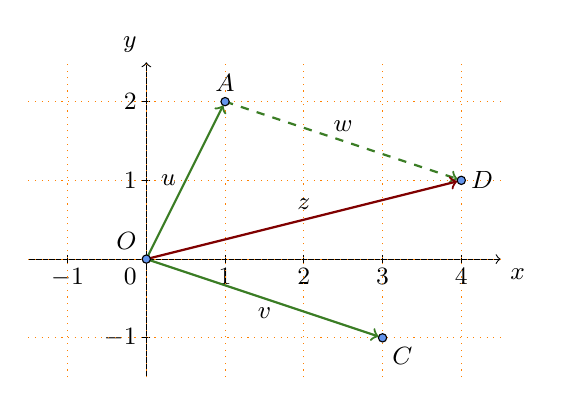
\begin{tikzpicture}[x=10mm,y=10mm, font=\small]

  \begin{scope}[->]
    \draw (-1.5,0) -- (4.5,0) node [below right] () {$x$};
    \draw (0,-1.5) -- (0,2.5) node[above left] {$y$};
  \end{scope}

  \foreach \x/\xtext in {-1/-1, 1/1,2/2,3/3,4/4}{
    \node[below] at (\x,0) {$\xtext$};
    \draw (\x,1.5pt) -- (\x,-1.5pt);}
  \foreach \y/\ytext in {-1/-1, 1/1,2/2}{
    \node[left] at (0,\y) {$\ytext$};
    \draw (1.5pt,\y) -- (-1.5pt,\y);}
  \node[below left] at (0,0) {$0$};

  \begin{scope}[dotted, orange]
    \draw (-1.5,-1.5) grid (4.5,2.5);
  \end{scope}

  \begin{scope}[thick, shorten >=1.5pt, ->]
  
	\draw[OliveGreen] (0,0) -- (1,2);
	\draw[OliveGreen] (0,0) -- (3,-1);
	\draw[OliveGreen, dashed] (1,2) -- (4,1);  
	\draw[Maroon] (-0,0) -- (4,1);
      \end{scope}
  
\begin{scope}[fill=CornflowerBlue, draw=black]
\filldraw (1,2) circle (1.5pt) node[above] {$A$};
\filldraw (0,0) circle (1.5pt) node[above left] {$O$};
\filldraw (4,1) circle (1.5pt) node[right] {$D$};
\filldraw (3,-1) circle (1.5pt) node[below right] {$C$};
\end{scope}

\node[left] at (.5,1) {$u$};
\node[above] at (2.5,1.5) {$w$};
\node[above] at (2,.5) {$z$};
\node[below] at (1.5,-.5) {$v$};
\end{tikzpicture}
\caption{Determinazione di componenti di un vettore.}\label{fig:F.10}
\end{figure}
\end{inaccessibleblock}

\begin{procedura} Regola del parallelogrammo per determinare le componenti 
cartesiane del vettore somma~$\vec{z}=(x_z;y_z)$,
note le componenti cartesiane degli addendi~$\vec{u}=(x_u;y_u)$ 
e~$\vec{v}=(x_v;y_v)$.

Il primo passo realizzato nella costruzione precedente ci permette di affermare 
che le componenti del vettore somma sono la somma
delle componenti dei vettori addendi:\[x_z=x_u+x_v\text{ e }y_z=y_u+y_v.\]
\end{procedura}

% \ovalbox{\risolvi \ref{ese:F.3}}

\paragraph{Applicazioni dei vettori}
I vettori sono degli enti geometrici, essi sono utilizzati in fisica per 
rappresentare tutte le grandezze che sono definite conoscendo modulo, direzione,
verso e punto di applicazione. Esempi di grandezze vettoriali sono: la 
velocità, l'accelerazione, la forza, la densità di corrente elettrica.

% \begin{exrig}
\begin{esempio}
Nella figura seguente è rappresentata una scatola vista dall'alto. Su di essa 
agiscono due forze; calcola la forza risultante in ognuno dei casi della figura,
sapendo che una forza misura~$4 \unit{N}$ e l'altra~$9 \unit{N}$.
\begin{center}
 % (c) 2012 Dimitrios Vrettos - d.vrettos@gmail.com

\begin{tikzpicture}[x=9mm,y=9mm, font=\small]
\tkzDefPoint(0,0){A}
\tkzDefShiftPoint[A](36:2){B}
\tkzDefShiftPoint[A](0:2){C}
\tkzDefShiftPoint[A](0:1.62){H}
\tkzDrawLine[add=0 and 0, thin](A,B)
\tkzDrawLine[add=0 and 0, thin, dashed](H,B)
\tkzDrawLine[thin, end=$r$](A,C)
\tkzLabelPoints[below](A,H)
\tkzLabelPoints[above](B)
\tkzDrawPoints[	color=CornflowerBlue](A,B, H)
\end{tikzpicture}
\end{center}
\emph{Svolgimento:}
\begin{enumeratea}
\item I due vettori hanno la stessa direzione e lo stesso verso quindi la 
risultante si ottiene addizionando i due moduli:~$|\vec{r}|=4 \unit{N}+9 
\unit{N}=13 \unit{N}$
\item poiché i vettori sono opposti come verso, si procede sottraendo al 
vettore maggiore il vettore minore e la forza risultante ha la direzione ed il 
verso
del vettore di modulo maggiore:~$|\vec{r}|=9 \unit{N} - 5 \unit{N}=4 \unit{N}$.
\item i due vettori hanno direzioni perpendicolari. In questo caso il vettore 
somma si ottiene con il metodo del parallelogrammo, quindi applicando il 
teorema di Pitagora:
\[|\vec{r}|=\sqrt{(4 \unit{N})^2+(9 \unit{N})^2}.\]
\end{enumeratea}
\end{esempio}
% \end{exrig}

\subsection{Differenza tra vettori}

\begin{procedura} Per determinare la \emph{differenza tra due vettori} 
(figura~\ref{fig:F.11}) $\vec{u}$ e~$\vec{v}$
si procede nel seguente modo:
\begin{enumeratea}
\item costruiamo il vettore~$\vec{z}=-\vec{v}$ che ha stessa direzione, stesso 
modulo, ma verso opposto;
\item determiniamo con la regola del parallelogrammo~$\vec{u}+\vec{z}=\vec{c}$.
\end{enumeratea}
Il vettore ottenuto è la differenza tra i vettori 
assegnati:~$\vec{c}=\vec{u}-\vec{v}$.
\end{procedura}

\begin{inaccessibleblock}[Differenza tra due fattori.]
 \begin{figure}[t]
 \centering
 % (c) 2012 Dimitrios Vrettos - d.vrettos@gmail.com

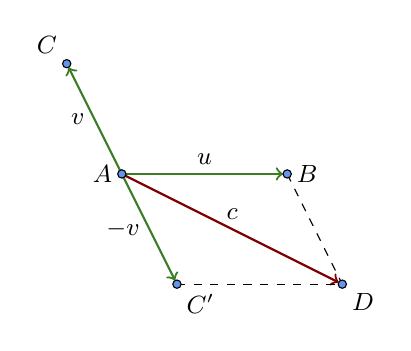
\begin{tikzpicture}[x=7mm,y=7mm, font=\small]

 \begin{scope}[thick, shorten >=1.5pt, ->]
  
	\draw[OliveGreen] (0,0) -- (-1,2);
	\draw[OliveGreen] (0,0) -- (1,-2);
	\draw[OliveGreen] (0,0) -- (3,0);  
	\draw[Maroon] (0,0) -- (4,-2);
      \end{scope}
  
\begin{scope}[dashed]
\draw (3,0) -- (4,-2);
\draw (1,-2) -- (4,-2);
\end{scope}
\begin{scope}[fill=CornflowerBlue, draw=black]
\filldraw (0,0) circle (1.5pt) node[left] {$A$};
\filldraw (3,0) circle (1.5pt) node[right] {$B$};
\filldraw (4,-2) circle (1.5pt) node[below right] {$D$};
\filldraw (1,-2) circle (1.5pt) node[below right] {$C'$};
\filldraw (-1,2) circle (1.5pt) node[above left] {$C$};
\end{scope}

\node[above] at (1.5,0) {$u$};
\node[above] at (2,-1) {$c$};
\node[left] at (.5,-1) {$-v$};
\node[left] at (-.5,1) {$v$};
\end{tikzpicture}
 \caption{Differenza di due vettori.}
 \label{fig:F.11}
\end{figure}
\end{inaccessibleblock}

% \begin{exrig}
\begin{esempio}

Sono assegnati i vettori~$\vec{u}(4;0)$ e~$\vec{v}(-2;-1)$. 
Determinare~$\vec{d_1}=\vec{u}-\vec{v}$ e~$\vec{d_2}=\vec{v}-\vec{u}$. Cosa 
osservate?
\begin{center}
 % (c) 2012 Dimitrios Vrettos - d.vrettos@gmail.com

\begin{tikzpicture}[x=10mm,y=10mm, font=\small]

  \begin{scope}[dotted, orange]
    \draw (-2.5,-1.5) grid (6.5,1.5);
  \end{scope}

  \begin{scope}[->]
    \draw (-2.5,0) -- (6.5,0) node [below right] {$x$};
    \draw (0,-1.5) -- (0,1.5) node[above left] {$y$};
  \end{scope}

  \foreach \x/\xtext in {-2/-2,-1/-1,1/1,2/2,3/3,4/4,5/5,6/6}{
    \node[below] at (\x,0) {$\xtext$};
    \draw (\x,1.5pt) -- (\x,-1.5pt);}
  \foreach \y/\ytext in {-1/-1, 1/1}{
    \node[left] at (0,\y) {$\ytext$};
    \draw (1.5pt,\y) -- (-1.5pt,\y);}
  \node[below left] at (0,0) {$0$};

  \begin{scope}[thick, ->,shorten >=1.5pt]
    \draw[Maroon] (0,0) -- (4,0);  
    \draw[OliveGreen](0,0) -- (-2,-1);
  \end{scope}

  \begin{scope}[fill=CornflowerBlue, draw=black]
    \filldraw (0,0) circle (1.5pt)node [above left]{$O$};
    \filldraw (4,0) circle (1.5pt)node [above right]{$A$};
    \filldraw (-2,-1) circle (1.5pt) node [below left]{$C$};
  \end{scope}
  
  \node[above] at (2,0) {$u$};
  \node[below] at (-1,-.5) {$v$};

\end{tikzpicture}
\end{center}
\end{esempio}
% \end{exrig}

\subsection{Moltiplicazione di un numero reale per un vettore}

\begin{definizione}
Assegnato un numero reale~$r$ ed un vettore~$\vec{v}$, il \emph{prodotto}~$r 
\cdot \vec{v}$ è un vettore~$\vec{p}$ avente:
\begin{enumeratea}
\item la stessa direzione del vettore~$\vec{v}$
\item intensità o modulo uguale al prodotto del modulo di~$\vec{v}$ per il 
valore assoluto di~$r$:
 \subitem $|\vec{p}|=|r| \cdot|\vec{v}|$
\item verso uguale al verso di~$\vec{v}$ se~$r$ è positivo, verso opposto a 
quello di~$\vec{v}$ se~$r$ è negativo.
\end{enumeratea}
\end{definizione}

% \begin{exrig}
\begin{esempio}
Nella figura sono rappresentati il vettore~$\vec{v}$ e altri vettori ottenuti 
moltiplicandolo per un numero reale:
$\vec{a}=2 \cdot \vec{v}$,$\vec{b}=-\dfrac{3}{2} \cdot \vec{v}$, 
$\vec{c}=\dfrac{1}{3} \cdot \vec{v}$.
\begin{center}
 % (c) 2012 Dimitrios Vrettos - d.vrettos@gmail.com

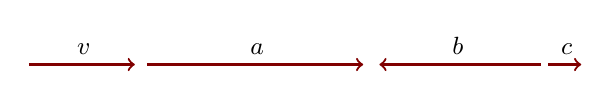
\begin{tikzpicture}[x=7mm,y=7mm, font=\small]

 \begin{scope}[thick, shorten >=1.5pt, ->, Maroon]
	\draw (0,0) -- (2,0); %vettore v
\node[above, black] at (1,0) {$v$};
	\begin{scope}[xshift=15mm]
	\draw (0,0) -- (4,0); %vettore a
\node[above, black] at (2,0) {$a$};
	\end{scope}
	\begin{scope}[xshift=44mm]
	\draw (3,0) -- (0,0); %vettore b
\node[above, black] at (1.5,0) {$b$};
	\end{scope}
	\begin{scope}[xshift=66mm]
	\draw (0,0) -- (.67,0); %vettore c
\node[above, black] at (.33,0) {$c$};
	\end{scope}
\end{scope}

\end{tikzpicture}
\end{center}

\end{esempio}
\begin{esempio}
Nel piano dotato di riferimento cartesiano ortogonale rappresentiamo il 
vettore~$\vec{u}(4;1)$ le componenti
del vettore~$\vec{p}=-2\cdot \vec{u}$ si ottengono moltiplicando per~$-2$ le 
componenti del vettore dato:~$\vec{p}(-8;-2)$. $\vec{p}$ e~$\vec{u}$
hanno la stessa direzione essendo~$m_{\vec{u}}=\frac{1}{4}=m_{\vec{p}}$ e anzi 
appartengono alla stessa retta avendo in comune il punto di applicazione.
\begin{center}
 % (c) 2012 Dimitrios Vrettos - d.vrettos@gmail.com

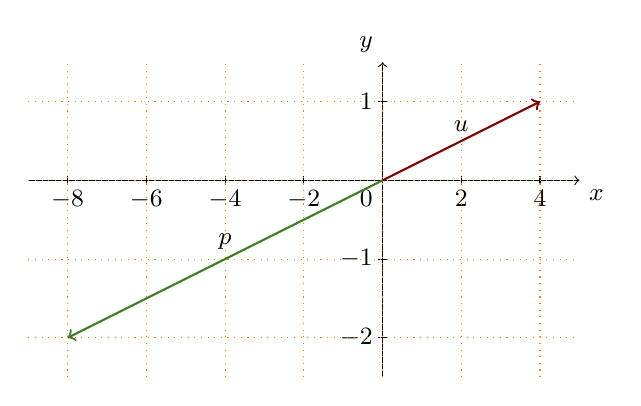
\begin{tikzpicture}[x=10mm,y=10mm, font=\small]

  \begin{scope}[->]
    \draw (-4.5,0) -- (2.5,0) node [below right] () {$x$};
    \draw (0,-2.5) -- (0,1.5) node[above left] {$y$};
  \end{scope}

  \foreach \x/\xtext in {-4/-8, -3/-6,-2/-4,-1/-2,1/2,2/4}{
    \node[below] at (\x,0) {$\xtext$};
    \draw (\x,1.5pt) -- (\x,-1.5pt);}
  \foreach \y/\ytext in {-2/-2,-1/-1, 1/1}{
    \node[left] at (0,\y) {$\ytext$};
    \draw (1.5pt,\y) -- (-1.5pt,\y);}
  \node[below left] at (0,0) {$0$};

  \begin{scope}[dotted, orange]
    \draw (-4.5,-2.5) grid (2.5,1.5);
  \end{scope}

  \begin{scope}[thick, ->]
	\draw[Maroon] (0,0) -- (2,1);  
	\draw[OliveGreen](0,0) -- (-4,-2);
      \end{scope}
 
\node[above] at (1,.5) {$u$};
\node[above] at (-2,-1) {$p$};
\end{tikzpicture}
\end{center}
\end{esempio}
% \end{exrig}

In generale~$\vec{u}(x_u;y_u) \rightarrow r \cdot \vec{u}=
             \vec{p}(r \cdot x_u; 
             r \cdot y_u)$ e~$m_{\vec{u}}=m_{\vec{p}}$.
   
\begin{osservazione}
Se due vettori hanno la stessa direzione, cioè appartengono a rette parallele 
(non coincidenti), si può sempre trovare un numero reale~$r$
tale che uno sia~$r$ volte l'altro. La figura seguente può suggerirvi come 
giustificare l'osservazione precedente.
\begin{center}
 % (c) 2012 Dimitrios Vrettos - d.vrettos@gmail.com

\begin{tikzpicture}[x=10mm,y=10mm, font=\small]

  \begin{scope}[->, thick]
\draw[OliveGreen] (0,0) -- (4,0);
\draw[Maroon] (1,1) -- (3,1);
\end{scope}
\node[above] at (2,1) {$u$};
\node[above] at (2,0) {$v$};
\begin{scope}[dotted]
\draw (0,0) -- (2,2)--(4,0);
\end{scope}
\end{tikzpicture}
\end{center}
\end{osservazione}

% \begin{exrig}
\begin{esempio}

Sono assegnati i vettori~$\vec{x}(\frac {1}{2};1)$ $\vec{y}(-3;-1)$ 
$\vec{z}(0;3)$.
Costruite i vettori:~$\vec{p_1}=2 \cdot \vec{x}-\vec{y}$\, $\vec{p_2}=2 \cdot 
(\vec{z}+\vec{y})$\, $\vec{p_3}=-\frac {3}{2} \cdot \vec{z} +2 \cdot \vec{y}+3 
\cdot \vec{x}$
e determinatene le componenti.
\end{esempio}
% \end{exrig}

\subsection{Il prodotto scalare}

Consideriamo due vettori $\vec{u}$ e $\vec{v}$ non nulli e 
sia~$\alpha$ l'angolo da essi formato.

\begin{inaccessibleblock}[Due vettori u e v e l'angolo compreso.]
 \begin{figure}[t]
 \centering
  % (c) 2012 Dimitrios Vrettos - d.vrettos@gmail.com
% (c) 2015 Daniele Zambelli - daniele.zambelli@gmail.com

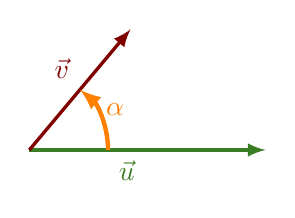
\begin{tikzpicture}[x=10mm,y=10mm, >=latex]

\begin{scope}[->, very thick]
\draw [OliveGreen] (0, 0) -- (1, 0) node [below right] {$\vec{u}$} --(3, 0);
\draw [Maroon] (0,0) -- (50:1) node [above left] {$\vec{v}$} -- (50:2);
\draw [->, ultra thick, orange] (1, 0) arc(0:50:1);
\end{scope}
\draw [orange] (0,0) (25:1.2) node {$\alpha$};

\end{tikzpicture}

% \begin{tikzpicture}[x=20mm,y=20mm, >=latex]
% 
% % Griglia
% \draw[gray!50, very thin, step=1] (-1.2, -1.2) grid (1.2, 1.2);
% 
% % (c) 2014 Daniele Zambelli - daniele.zambelli@gmail.com

%%%
% Circonferenza goniometrica
%%%%
% 
% % Griglia
% \draw[gray!50, very thin, step=1] (-1.2, -1.2) grid (1.2, 1.2);

%Asse x
\draw [-{Stealth[length=2mm, open, round]}] (-1.3,0) -- (1.3,0) node [below]
      {$x$};
%Asse y
\draw [-{Stealth[length=2mm, open, round]}] (0, -1.3) -- (0, 1.3) node [left]  
      {$y$};
%Circonferenza
\draw [very thin] (0,0) circle (1);

% 
% \begin{scope}[->, very thick]
% \draw [Maroon!50!black, rotate=65] (0,0)--(1,0 );
% \draw [orange] (0, 0) (20:1.3) arc (20:70:1.3);
% \draw [orange] (0, 0) (160:1.3) arc (160:110:1.3);
% \draw [green!50!black] (.3, 0) arc(0:65:.3);
% \draw [green!50!black] (1, 0) arc(0:65:1);
% \end{scope}
% 
% \draw [black] (1.1, 1.1) node {$+$};
% \draw [black] (-1.1, 1.1) node {$-$};
% 
% \begin{tikzpicture}[x=10mm,y=10mm, font=\small]
% 
%   \begin{scope}[thick,shorten >=1.5pt, ->]
%     \begin{scope}[OliveGreen]
%       \draw (0,0) -- (2,1);
%       \draw (0,0) -- (3,-1);
%     \end{scope}  
%     
%     \begin{scope}[Maroon]
%       \draw (0,0) -- (5,0);
%     \end{scope}
%   \end{scope}
% 
%   \begin{scope}[dashed]
%     \draw[xshift=30mm,yshift=-10mm] (0,0) -- (2,1);
%     \draw[xshift=20mm,yshift=10mm] (0,0) -- (3,-1);
%   \end{scope}
% 
%   \begin{scope}[fill=CornflowerBlue, draw=black]
%     \filldraw (5,0) circle (1.5pt) node[right] {$D$};
%     \filldraw (0,0) circle (1.5pt) node[left] {$A$};
%     \filldraw (2,1) circle (1.5pt) node[above] {$B$};
%     \filldraw (3,-1) circle (1.5pt) node[below] {$C$};
%   \end{scope}
% 
%   \node[above] at (2.5,0) {$w$};

% \end{tikzpicture}
 \caption{Prodotto scalare tra due vettori.}
 \label{fig:vett_prodotto_scalare}
\end{figure}
\end{inaccessibleblock}
                  
Il prodotto scalare può assumere valore positivo, negativo o nullo a seconda 
dell'angolo~$\alpha$ che i due vettori $\vec{u}$ e $\vec{v}$ non nulli formano. 
In particolare:
\begin{itemize}
 \item se i vettori $\vec{u}$ e $\vec{v}$ sono paralleli e 
  quindi $\alpha=0\grado$
  \[\vec{u} \cdot \vec{v} = \lvert\vec{u}\rvert\lvert\vec{v}\rvert \cos \alpha=
    \lvert\vec{u}\rvert\lvert\vec{v}\rvert\] 
  in quanto $\cos 0\grado = 1$;
 \item se i vettori $\vec{u}$ e $\vec{v}$ sono perpendicolari e 
  quindi $\alpha=90\grado$
  \[\vec{u} \cdot \vec{v} = 0\] 
  in quanto $cos 90\grado = 0$;
 \item in tutti gli altri casi dipende dal valore di $\cos \alpha$ che è 
  positivo se $-90\grado < \alpha < +90\grado$ e negativo 
  se $+90\grado < \alpha < 270\grado$
\end{itemize}

% \begin{exrig}
 \begin{esempio}
  Calcola il prodotto scalare dei  vettori $\vec{u}$ e $\vec{v}$, 
  che hanno moduli $\lvert\vec{u}\rvert= 3 \text{ e } \lvert\vec{v}\rvert=5$ 
  e che formano un angolo di $120\grado$.
  \[\vec{u} \cdot \vec{v} = 
    \lvert\vec{u}\rvert\lvert\vec{v}\rvert \cos \alpha=
    3 \cdot 5 \cdot \cos 120\grado = 15 \cdot \left(-\frac{1}{2} \right)=
    -7,5\]
 \end{esempio}

 \begin{esempio}
  Calcola il prodotto scalare dei  vettori $\vec{u}$ e $\vec{v}$, 
  che hanno moduli $\lvert\vec{u}\rvert= 3 \text{ e } \lvert\vec{v}\rvert=6$ 
  e che formano un angolo di~$60\grado$.
  \[\vec{u} \cdot \vec{v} = 
    \lvert\vec{u}\rvert\lvert\vec{v}\rvert \cos \alpha=
    4 \cdot 7 \cdot \cos 60\grado = 28 \cdot \left(\frac{1}{2} \right)=
    +14\]
 \end{esempio}

% \end{exrig}

\subsubsection{Proprietà}

Il prodotto scalare gode delle seguenti proprietà:
\begin{itemize}
 \item proprietà \emph{commutativa}:
  \[\vec{u} \cdot \vec{v} = \vec{v} \cdot \vec{u}\]
 \item proprietà \emph{distributiva} rispetto alla somma di vettori:
  \[\left(\vec{u} + \vec{v} \right) \cdot \vec{w} = 
    \vec{u} \cdot \vec{w} + \vec{v} \cdot \vec{w}\]
 \item proprietà \emph{associativa}:
  \[\left(\vec{u} \cdot \vec{v} \right) \cdot \vec{w} = 
    \vec{u} \cdot \left(\vec{v} \cdot \vec{w} \right)\]
\end{itemize}

\subsubsection{Prodotto scalare nel piano cartesiano}

È possibile esprimere il prodotto scalare di due 
vettori~$\vec{u}=(x_u;~y_u)$ e $\vec{v}=(x_v;~y_v)$ 
in funzione delle loro componenti tramite la formula:
\[\vec{u} \cdot \vec{v} = x_u x_v + y_u y_v\]

 \begin{esempio}
  Calcola il prodotto scalare dei vettori $\vec{a}(3;~5)$ e $\vec{b}(4;~-2)$.
\[\vec{a} \cdot \vec{b} = x_a x_b + y_a y_b = 3 \cdot 4 + 5 \cdot (-2)= 
  12-10 = 2\]
 \end{esempio}

\subsection{Il prodotto vettoriale}

I matematici hanno anche inventato una ``moltiplicazione'' tra due vettori che
dà come risultato un vettore e la hanno chiamata prodotto vettoriale.

% \begin{wrapfloat}{figure}{r}{0pt}
% \includegraphics[scale=0.35]{img/fig000_.png}
% \caption{...}
% \label{fig:...}
% \end{wrapfloat}

\begin{inaccessibleblock}[Due vettori u e v e il prodotto vettoriale.]
 \begin{figure}[h]
 \centering
  % (c) 2014 Daniele Zambelli - daniele.zambelli@gmail.com

\newcommand{\duevettori}[2]{%
  \draw [rounded corners, fill, blue!30] 
      (-1, -0.5) -- (4, -0.5) -- (6, 1.5) -- (1, 1.5) -- cycle;
  \begin{scope}[->, very thick]
    \draw [OliveGreen] (0, 0) -- (2, 0) node [below right] {$\vec{u}$} -- 
        (4, 0);
    \draw [Maroon] (0, 0) -- (20:2) node [above left] {$\vec{v}$} -- 
        (20:3);
    \draw [blue!60!black] (0, 0) -- 
        (0, #1 * 1) node [left] {#2} --
        (0, #1 * 2);
    \draw [-, orange] (1.5, 0) arc(0:20:1.5);
  \end{scope}
  \draw [orange] (0,0) (10:1.8) node {$\alpha$};
}

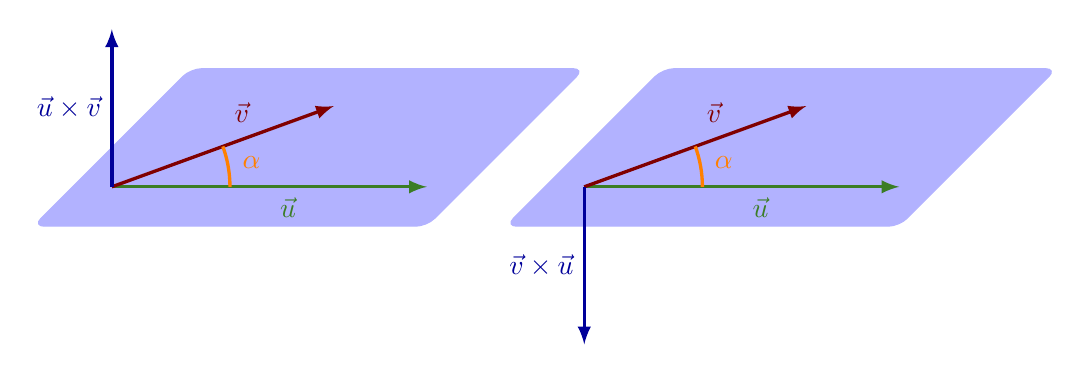
\begin{tikzpicture}[x=10mm,y=10mm, >=latex]

\begin{scope}[shift={(-5, 0)}]
\duevettori{+1}{$\vec{u} \times \vec{v}$}
\end{scope}

\begin{scope}[shift={(+1, 0)}]
\duevettori{-1}{$\vec{v} \times \vec{u}$}
\end{scope}

\end{tikzpicture}

 \caption{Prodotto vettoriale tra due vettori.}
 \label{fig:vett_prodotto_vettoriale}
\end{figure}
\end{inaccessibleblock}

Consideriamo due vettori $\vec{u}$ e $\vec{v}$ non nulli e 
sia~$\alpha$ l'angolo da essi formato.

\begin{definizione}
 Si dice \emph{prodotto vettoriale} $\vec{u} \times \vec{v}$
 e si legge ``u vettore v'' il vettore che ha: 
 \begin{itemize}
  \item \emph{modulo} uguale 
   a~$\lvert\vec{u}\rvert\lvert\vec{v}\rvert \sin \alpha$
  \item direzione perpendicolare al piano individuato dai due 
   vettori $\vec{u}$ e $\vec{v}$
  \item \emph{verso} quello in cui avanza una vite normale (destrorsa) 
   cioè una vite che si avvita ruotandola in senso orario
   fatta ruotare nel senso di rotazione che porta $\vec{u}$ su $\vec{v}$.
 \end{itemize}
\end{definizione}
 
In particolare:
\begin{itemize}
 \item se i vettori $\vec{u}$ e $\vec{v}$ sono paralleli e 
  quindi $\alpha=0\grado$
  \[\vec{u} \times \vec{v} = \lvert\vec{u}\rvert\lvert\vec{v}\rvert \sin \alpha=
    \lvert\vec{u}\rvert\lvert\vec{v}\rvert \sin 0\grado=0\] 
  in quanto $\sin 0\grado = 0$;
 \item se i vettori $\vec{u}$ e $\vec{v}$ sono perpendicolari e 
  quindi $\alpha=90\grado$
  \[\vec{u} \times \vec{v} = \lvert\vec{u}\rvert\lvert\vec{v}\rvert \sin \alpha=
    \lvert\vec{u}\rvert\lvert\vec{v}\rvert\]
  in quanto $sin 90\grado = 1$
\end{itemize}

 \begin{esempio}
  Calcola il prodotto vettoriale dei  vettori $\vec{u}$ e $\vec{v}$, 
  che hanno moduli $\lvert\vec{u}\rvert= 3 \text{ e } \lvert\vec{v}\rvert=7$ 
  e che formano un angolo di $60\grado$. 
 \begin{itemize}
  \item \emph{modulo} uguale 
  \[\vec{u} \times \vec{v} = 
    \lvert\vec{u}\rvert\lvert\vec{v}\rvert \sin \alpha=
    3 \cdot 7 \cdot \sin 60\grado = 21 \cdot \frac{1}{2} = 10,5\]
  \item direzione perpendicolare al piano individuato dai due 
   vettori $\vec{u}$ e $\vec{v}$
  \item \emph{verso} entrante nel piano.
 \end{itemize}
 \end{esempio}


\osservazione
È importante notare  che il modulo del prodotto vettoriale è uguale all'area 
del parallelogramma che ha per lati i due vettori.
Infatti, come si può vedere dalla figura \ref{fig:vett_parallelogramma}      

\begin{inaccessibleblock}[Parallelogramma con evidenziati i lati come vettori
  e l'altezza.]
 \begin{figure}[h]
 \centering
  % (c) 2014 Daniele Zambelli - daniele.zambelli@gmail.com

\newcommand{\parallelogramma}[3]{%
  \def \pu{#1}
  \def \palpha{#2}
  \def \pv{#3}
  \coordinate (a) at (0, 0);
  \coordinate (b) at (\pu, 0);
  \coordinate (d) at (\palpha:\pv);
  \coordinate (h) at (d |- b);
  \coordinate (c) at ([xshift=\pu cm] d); % se cambia la scala questo punto sballa
  \begin{scope}[black]
    \draw (a) node [below left] {$A$};
    \draw (b) node [below right] {$B$};
    \draw (c) node [above right] {$C$};
    \draw (d) node [above left] {$D$};
    \draw (h) node [below] {$H$};
  \end{scope}
%   \draw [fill, green!50] 
%       (0, 0) --++ (\u, 0) --++ (\alpha:\v) --++ (-\u, 0) -- cycle;
  \draw [fill, green!50] (a) -- (b) -- (c) -- (d) -- cycle;
  \begin{scope}[very thick]
    \draw [->, OliveGreen!80!black] (0, 0) -- node [below right] {$\vec{u}$} (b);
    \draw [->, Maroon!80!black] (0, 0) -- node [above left] {$\vec{v}$} (d);
    \draw [gray, dashed] (d) -- node [right] {$h=v \cdot \sin \alpha$} (h);
    \draw [orange!80!black] (0.5, 0) arc(0:\palpha:0.5);
    \draw [orange!80!black] (0,0) (\palpha / 2:0.8) node {$\alpha$};
  \end{scope}
}

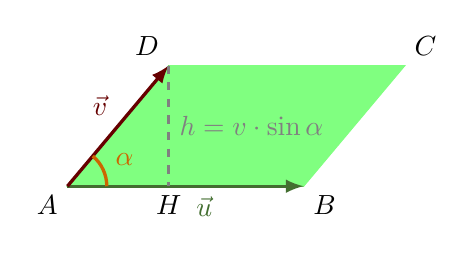
\begin{tikzpicture}[x=10mm,y=10mm, >=latex]

\parallelogramma{3}{50}{2}

\end{tikzpicture}

 \caption{Area del parallelogramma e modulo del prodotto vettoriale.}
 \label{fig:vett_parallelogramma}
\end{figure}
\end{inaccessibleblock}

\[Area (ABCD)=\overline{AB} \cdot \overline{DH} =
            \overline{AB} \cdot \overline{AD} \sin \alpha =
            \lvert\vec{u}\rvert\lvert\vec{v}\rvert \sin \alpha=
            \vec{u} \times \vec{v}\]

\subsubsection{Proprietà}

Proprietà:
\begin{itemize}
 \item il prodotto vettoriale \emph{non} gode della proprietà 
  \emph{commutativa} infatti:
  \[\vec{u} \times \vec{v} = - \vec{v} \times \vec{u}\]
 \item gode della proprietà \emph{distributiva} rispetto alla somma di vettori:
  \[\left(\vec{u} + \vec{v} \right) \times \vec{w} = 
    \vec{u} \times \vec{w} + \vec{v} \times \vec{w}\]
 \item gode della proprietà \emph{associativa} rispetto alla moltiplicazione
  per uno scalare:
  \[\left(k \cdot \vec{u} \right) \times \vec{v} = 
    k \cdot \left(\vec{u} \times \vec{v} \right)\]
\end{itemize}

% \ovalbox{\risolvii \ref{ese:F.4}, \ref{ese:F.5}, \ref{ese:F.6}}

% \section{Dipendenza e indipendenza lineare}
% \begin{definizione}
% Diciamo che un vettore~$\vec{v}$ è \emph{combinazione lineare} di altri 
% vettori~$\vec{x}; \vec{y}; \vec{z}$ se vale
% l'uguaglianza~$\vec{v}=r_1 \cdot \vec{x} + r_2 \cdot \vec{y} + r_3 \cdot 
% \vec{z}$ i numeri reali~$r_1, r_2, r_3$
% sono i coefficienti della combinazione lineare.
% \end{definizione}
% \newpage
% \begin{exrig}
% \begin{esempio}
% Nell'esempio precedente hai costruito i vettori~$\vec{p_1}; \vec{p_2}; 
% \vec{p_3}$ eseguendo la somma algebrica di vettori costruiti moltiplicando
% per numeri reali i vettori assegnati~$\vec{x}; \vec{y}; \vec{z}$. Possiamo 
% dire che:
% \begin{itemize*}
% \item $\vec{p_1}$ è combinazione lineare dei vettori~$\vec{x}$ e~$\vec{y}$ i 
% cui 
% coefficienti sono~$r_1=2, r_2=-1$.
% \item $\vec{p_2}$ è combinazione lineare dei vettori~$\vec{z}$ e~$\vec{y}$ i 
% cui 
% coefficienti sono~$r_1=2, r_2=2$.
% \item $\vec{p_3}$ è combinazione lineare dei vettori~$\vec{x}$,$\vec{y}$ 
% e~$\vec{z}$ i cui coefficienti sono~$r_1=-\frac{3}{2}, r_2=2, r_3=3$.
% \end{itemize*}
% \end{esempio}
% \end{exrig}
% 
% Nell'insieme~$\spV$ di tutti i vettori del piano cartesiano, consideriamo i 
% vettori~$\vec{i}(1;0)$ e~$\vec{j}(0;1)$ rispettivamente appartenenti
% all'asse delle ascisse e delle ordinate; possiamo notare che
% \[|\vec{i}|=|\vec{j}|=1.\]
% 
% Ora, ogni vettore~$\vec{v}$ del piano può essere scritto come combinazione 
% lineare di~$\vec{i}$ e~$\vec{j}$ le sue componenti sono i coefficienti
% della combinazione lineare con cui si determina~$\vec{v}$.
% \[\vec{v}(x_v;y_v)=x_v \cdot \vec{i}+y_v \cdot \vec{j}\]
% 
% \ovalbox{\risolvi \ref{ese:F.7}}
% 
% \begin{exrig}
% \begin{esempio}
% Disegniamo nel riferimento cartesiano ortogonale i vettori~$\vec{u}(1;1)$, 
% $\vec{v}(4;-2)$, $\vec{w}(3;1)$ ci chiediamo se è possibile scrivere~$\vec{w}$
% come combinazione lineare degli altri due.
% \begin{center}
%  % (c) 2012 Dimitrios Vrettos - d.vrettos@gmail.com

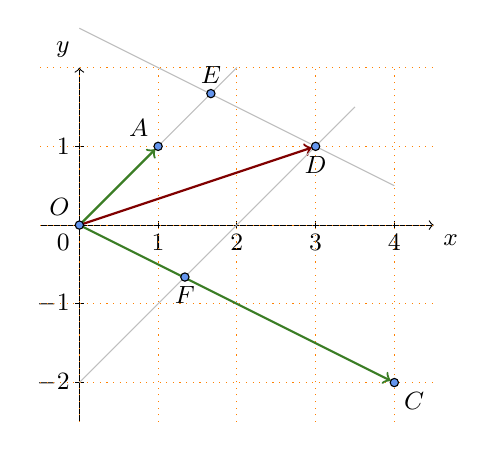
\begin{tikzpicture}[x=10mm,y=10mm, font=\small]

  \begin{scope}[->]
    \draw (-.5,0) -- (4.5,0) node [below right] {$x$};
    \draw (0,-2.5) -- (0,2) node[above left] {$y$};
  \end{scope}

  \foreach \x/\xtext in {1/1,2/2,3/3,4/4}{
    \node[below] at (\x,0) {$\xtext$};
    \draw (\x,1.5pt) -- (\x,-1.5pt);}
  \foreach \y/\ytext in {-2/-2,-1/-1, 1/1}{
    \node[left] at (0,\y) {$\ytext$};
    \draw (1.5pt,\y) -- (-1.5pt,\y);}
  \node[below left] at (0,0) {$0$};

  \begin{scope}[dotted, orange]
    \draw (-.5,-2.5) grid (4.5,2);
  \end{scope}

  \begin{scope}[thick, ->,shorten >=1.5pt]
	\draw[Maroon] (0,0) -- (3,1);  
	\draw[OliveGreen](0,0) -- (1,1);
	\draw[OliveGreen](0,0) -- (4,-2);
      \end{scope}
 
\begin{scope}[lightgray]
\draw (1,1) -- (2,2);
\draw[xshift=20mm] (-2,-2) -- (1.5,1.5);
\draw[yshift=25mm](0,0)--(4,-2);
\end{scope}

\begin{scope}[fill=CornflowerBlue, draw=black]
\filldraw (0,0) circle (1.5pt)node [above left]{$O$};
\filldraw (3,1) circle (1.5pt)node [below]{$D$};
\filldraw (1,1) circle (1.5pt)node [above left]{$A$};
\filldraw (1.34,-.66) circle (1.5pt)node [below]{$F$};
\filldraw (1.67,1.67) circle (1.5pt) node [above]{$E$};
\filldraw (4,-2) circle (1.5pt) node [below right]{$C$};

\end{scope}
\end{tikzpicture}
% \end{center}
% 
% 
% \paragraph{Il metodo geometrico} Dobbiamo costruire due vettori~$\vec{u}'=r_1 
% \cdot \vec{u}$ e~$\vec{v}'=r_2 \cdot \vec{v}$ tali che sommati diano
% il vettore~$\vec{w}$. Dal punto~$D$ tracciamo la parallela alla retta~$OC$, 
% che 
% interseca la retta~$AO$ nel punto~$E$ dallo stesso punto~$D$
% tracciamo la parallela alla retta~$AO$ che interseca in~$F$ la retta~$OC$. I 
% punti~$E$ ed~$F$ sono gli
% estremi dei due vettori~$\overrightarrow{OE}=r_1 \cdot \vec{u}$ 
% e~$\overrightarrow{OF}=r_2 \cdot \vec{v}$ con~$r_1>1$ e~$r_2<1$ 
% rispettivamente 
% ottenuti
% allungando e accorciando~$\vec{u}$ e~$\vec{v}$: si ha~$\vec{w}=r_1 \cdot 
% \vec{u} 
% + r_2 \cdot \vec{v}$.
% 
% \paragraph{Il metodo algebrico} Dobbiamo trovare due numeri~$r_1$ e~$r_2$ 
% tali 
% che
% \[ \vec{w}=r_1 \cdot \vec{u}+r_2 \cdot \vec{v} \rightarrow
% \left\{\begin{array}{l}
% 3=1 \cdot r_1+1 \cdot r_2 \\
% 1=1 \cdot r_1-2 \cdot r_2
% \end{array}\right. \]
% \newpage
% e risolvendo si ottiene~$r_1=\frac{5}{3}$ e~$r_2=\frac{1}{3}$, coerentemente 
% ai 
% risultati della costruzione effettuata.
% \end{esempio}
% \end{exrig}
% 
% \ovalbox{\risolvi \ref{ese:F.8}}
% 
% \begin{definizione}
% Dato un insieme~$V$ di vettori, questi si dicono \emph{linearmente 
% indipendenti} 
% se almeno uno di essi si può scrivere come combinazione lineare 
% degli altri.
% Altrimenti si dicono \emph{linearmente indipendenti}.
% \end{definizione}
% \osservazione "Altrimenti" nella definizione significa che nessun vettore 
% dell\'insieme può essere scritto come combinazione lineare degli altri.
% 
% \vspazio\ovalbox{\risolvii \ref{ese:F.9}, \ref{ese:F.10}}
